\textbf{Name:} Parick Harvey\\

\medskip

\textbf{Conspirators:} Christopher O'Neil for moral support

\medskip
\medskip

\hrule

\medskip


\assignmentsonly{\pleasesubmitprojectdraft}

\begin{enumerate}

\item 
  Tokunaga's law implies Horton's laws:

  In lectures, we established the following:
  $$
  n_\om
  =
  \underbrace{\textcolor{red}{2}\, n_{\om+1}}_{\rm generation}
  +
  \sum_{\om'=\om+1}^{\Om}
  \underbrace{\textcolor{red}{T_{\om'-\om}}\, n_{\om'}}_{\rm absorption}
  $$
  From here, derive Horton's law for stream numbers: $n_{\om}/n_{\om+1} = R_n$,
  where $R_n > 1$ and is independent of $\om$, and find
  $R_n$ in terms of Tokunaga's two parameters $T_1$ and $R_T$.

  
   \solutionstart
   \begin{align}
   T_{k} &= T_{1} R_{t}^{k-1}\\
   \text{let } k &= \omega\mathsf{'}-\omega\\
   \Rightarrow T_{\omega\mathsf{'}-\omega} &=
        T_{1}
        R_{t}^
            {\omega\mathsf{'}-\omega}
    \end{align}

\clearpage

    \begin{align}
    n_\omega &=
        2n_{\omega+1} +
        \sum^
            {\Omega}_
            {\omega\mathsf{'}=\omega+1}{
            T_{\omega\mathsf{'}-\omega}
            n_{\omega\mathsf{'}
            }}
        \\
    &=
        2n_{\omega+1} +
        \sum^
        {\Omega}_
        {\omega\mathsf{'}=\omega+1}{
            T_{1}
            R_{t}^{k-1}
            n_{\omega\mathsf{'}}
        }\\
    n_{\omega} &=
        2n_{\omega+1} +
        \sum^
        {\Omega-\omega}_
        {k=1}{
            T_{1}
            R_{t}^{k-1}
            n_{k+\omega}
        }\\
    \frac{n_{\omega}}{n_{\omega+1}} &=
        \frac{
            2n_{\omega+1}
            }{
            n_{\omega+1}
            } +
        \sum^
        {\Omega-\omega}_
        {k=1}{
            T_{1}
            R_{t}^{k-1}
            n_{k+\omega}
        }\\
    &= 2 +
        \sum^
        {\Omega-\omega}_
        {k=1}{
            T_{1}
            R_{t}^{k-1}
            n_{k+\omega}
        }\\
    &= 2 +
        \sum^
        {\Omega-\omega}_
        {k=1}{
            T_{1}
            R_{t}^{k-1}
            \left(
            R_{n}^{-(k-1)}
            \right)
        }\\
    &= 2 +
        \sum^
        {\infty}_
        {k=1}{
            T_{1}
            R_{t}^{k-1}
            \frac{
            n_{k+\omega}}
            {n_{\omega+1}}
        }\\
    &= 2 + T_{1}
        \sum^
        {\infty}_
        {k=1}{
            \frac{
            R_{t}}{
            R_{n}}^{k-1}
        }\\
    \end{align}

Given the ratios $R_t$ and $R_n$ we will assume $\frac{R_{t}}{R_{n}}^{k-1} < 1$.

    \begin{align}
    &= 2 + T_{1}
    \left(
        \frac
        {1}
        {1 - \frac{R_{t}} {R_{n}}}
    \right)\\
    &= 2 + T_{1}
    \frac
    {1}
    {1 - \frac{R_{t}} {R_{n}}} = R_n\\
    1 - \frac{R_{t}} {R_{n}}
    \Bigg(
        R_n - 2 &= T_1
            \left(
            \frac
            {1}
            {1 - \frac{R_{t}} {R_{n}}}
            \right)
    \Bigg)\\
    R_{n}
    \Bigg(
        (R_n - 2)
        \left(
            \frac{1}
            {1-\frac{R_{t}}{R_{n}}}
        \right) &= T_1
    \Bigg)\\
    \Rightarrow
    (R_n - 2)
    (R_n - R_t)
    &= T_1 R_n\\
    \Rightarrow
    R_{n}^{2}
    - 2R_n
    - R_t R_n
    + 2R_t
    &= T_1 R_n\\
    \Rightarrow
    R_{n}^{2} - 
    \left(
    2 + R_t + T_1
    \right)
    R_n + 2R_t
    &= 0
    \end{align}
    
Given the quadratic form from (19):\\
$$  
    R_n = \frac
    {2 + R_t + T_1 \pm \sqrt{(2+R_t+T_1)^2}-4(2R_t)}
    {2}
$$

and the values from the previous assignment: $R_t = 2$ and $T_1 = 2$:\\
$$
    R_n = \frac{6 \pm \sqrt{6^2-16}}{2} = 3 \pm \sqrt{5}
$$
    \solutionend

\item 

  Show $R_n = R_a$ by 
  using Tokunaga's law to find the average area of an
  order $\omega$ basin, $\bar{a}_\omega$, in terms
  of the average area of basins of order 1 to $\omega-1$.

  (In lectures, we use Horton's laws to roughly demonstrate
  this result.)

  %% Reminder: Tokunaga's law is 
  %% $$ T_{\omega,\omega'} = T_1 R_T^{\ \omega-\omega'-1} \quad
  %% \mbox{where} \quad \omega > \omega'.$$

  Here's the set up:
  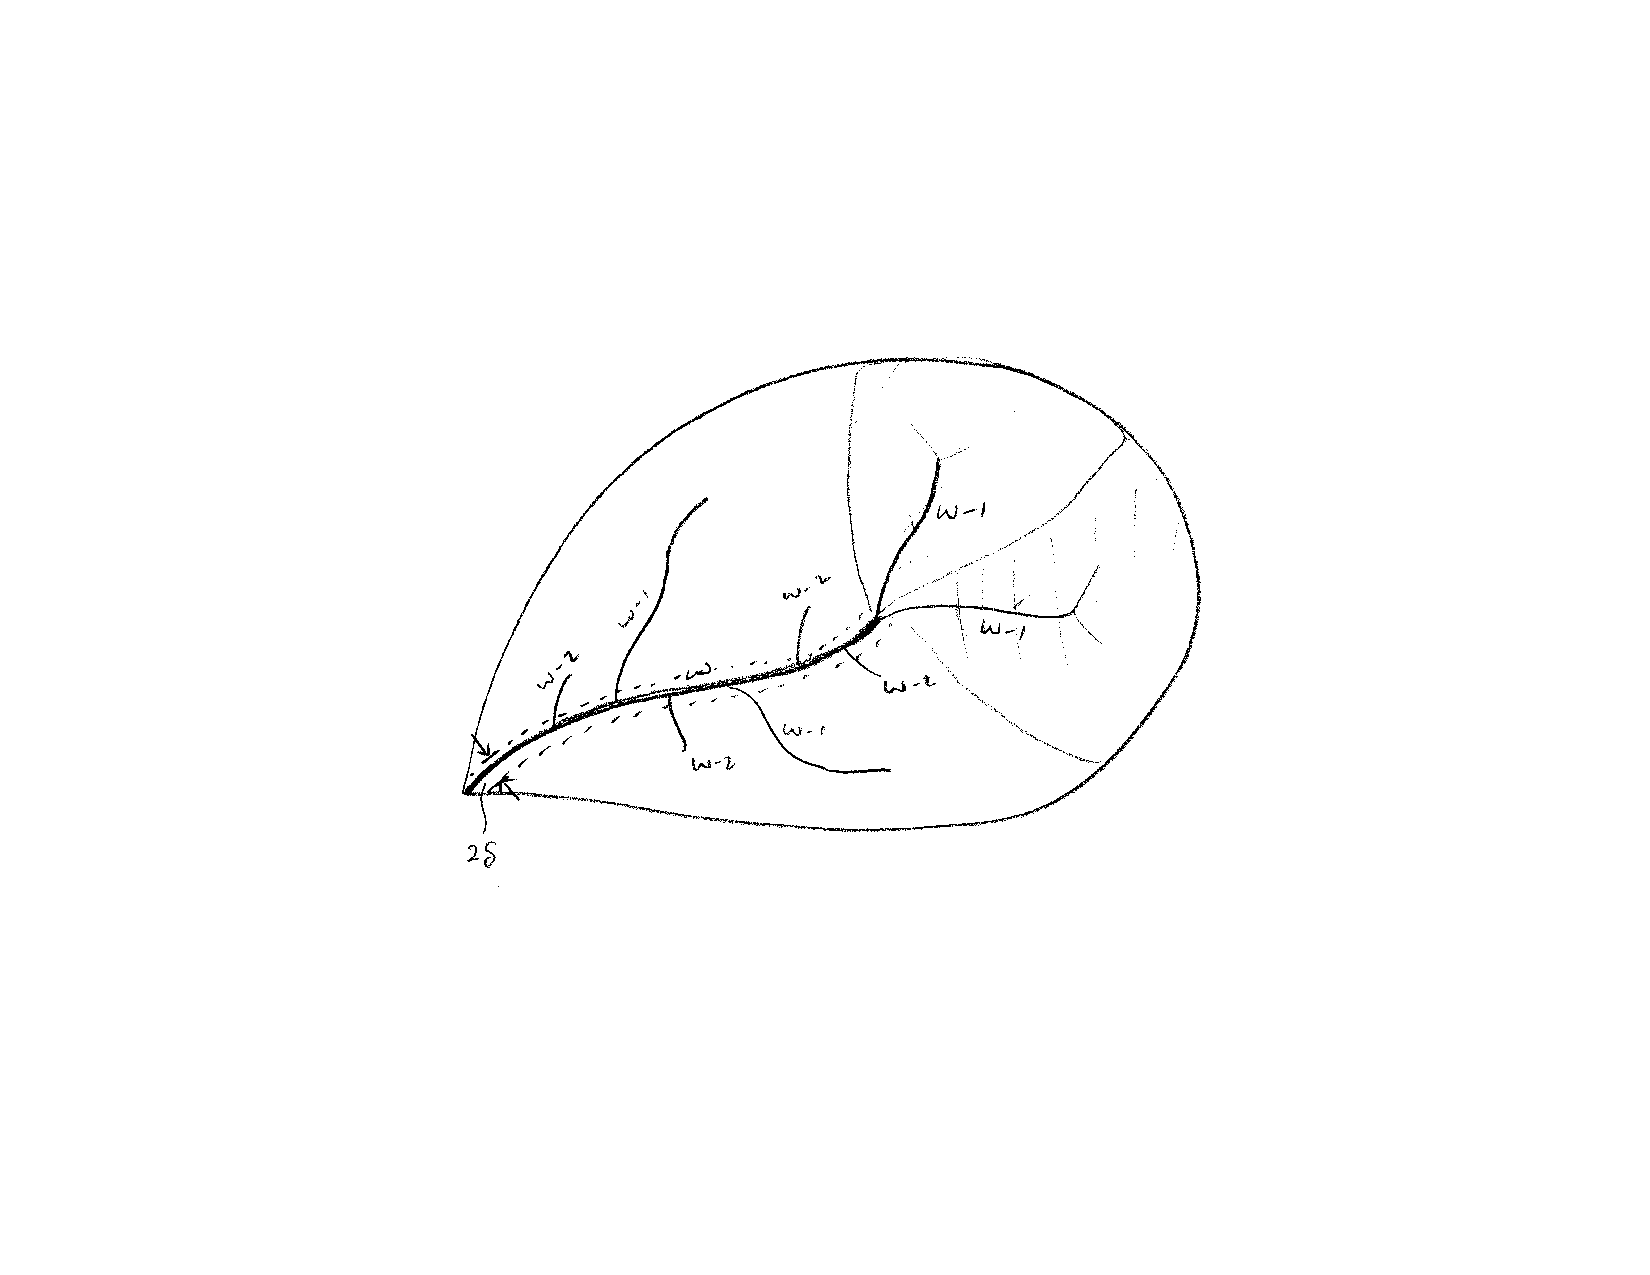
\includegraphics[width=0.8\textwidth]{ass1fig1.pdf}

  Using the Tokunaga picture, we see a basin of order $\om$ 
  can be broken down into non-overlapping sub-basins.

  Connect $\bar{a}_\om$ to the average areas of
  basins of lower orders as follows:
  $$
  \bar{a}_\om
  = 
  2\bar{a}_{\om-1}
  +
  \sum_{\om'=1}^{\om-1}
  T_{\om,\om'} 
  \bar{a}_{\om'}
  +
  2\delta \bar{\okell}_\om.
  $$
  The first term on the right hand side 
  corresponds to the two `generating' streams
  of order $\om-1$.  The second term (the sum)
  accounts for side streams entering the
  sole order $\om$ stream segment in the basin.
  And the last term gives the contribution of
  `overland flow,' i.e., flow that does not
  arrive in the main stream segment through
  a stream.  The length scale $\delta$ is
  the typical distance from stream to ridge.

  
   \solutionstart
   
   Given:
   \begin{align}
   \bar{a}_\om
   &= 
   2\bar{a}_{\om-1} +
   \sum_{\om'=1}^{\om-1}
   T_{\om,\om'} 
   \bar{a}_{\om'}
   +
   2\delta \bar{\okell}_\om\\
   T_{\om,\om'} &= T_1 R_{t}^{\om-\om'-1}\\
   \bar{a}_\om &= R_{a}^{\om-1} \bar{a}_1\\
   \bar{\okell_\om} &= R_{\okell}^{\om-1} \bar{\okell}_1\\
   \end{align}
   
   We can proceed as follows:
   
   \begin{align}
   \bar{a}_{1}\R^{\om-1}_{a}
   =
   2\bar{a}_{1}\R^{\om-2}_{a}
   +
   2\delta \bar{\okell}_1 R_{\okell}^{\om-1}
   &+
   T_1 \bar{a}_{1}
   \sum_{\om'=1}^{\om-1}
   R_{t}^{\om-\om'-1}
   R_{a}^{\om'-1}\\
   1
   =
   \frac{2} {R_a}
   +
   {2\delta \bar{\okell}_1} {\bar{a}_1}
   \left(
   \frac{R_s}{R_a}
   \right)^{\om-1}
   &+
   T_1
   \sum_{\om'=1}^{\om-1}
   R_{t}^{\om-\om'-1}
   R_{a}^{\om'-\om}\\
   &= 
   \frac{2} {R_a}
   +
   T_1
   \sum_{\om'=1}^{\om-1}
   R_{t}^{\om-\om'-1}
   R_{a}^{\om'-\om}\\
   1 &= 
   \frac{2} {R_a}
   +
   T_1
   \sum_{\om'=1}^{\om-1}
   R_{t}^{\om-\om'-1}
   R_{a}^{-(\om-\om')}
   \end{align}

Letting $i = (\om-\om')$\\

   \begin{align}
   &= 
   \frac{2} {R_a}
   +
   \frac{T_1}{R_a}
   \sum_{i=1}^{\om-1}
   \left(
        \frac{R_{t}}{R_a}
   \right)^{i}
   \end{align}

Assuming  $|\frac{R_t}{R_a}| > 1$\\
$$
   1 = \frac{R_t T_1}{R_a (R_a - R_t)} + \frac{2}{R_a}
$$

$$
   R_a = 2, R_t = \pm 1, T_1 = 0
$$
   
   \solutionend

\item 

  For river networks, basin areas are distributed
  according to $P(a) \propto a^{-\tau}$.

  Determine the exponent $\tau$ in terms of the Horton ratios
  $R_n$ and $R_\okell$.

  Guide:

  Follow the same procedure shown in lectures for
  $P(\ell) \propto \ell^{-\gamma}$.

    In class, we derived $P(\msl) \propto \msl^{-\gamma}$ starting
    from Horton's laws (see the section of scaling relations
    in the slides on Branching Networks II.
    In doing so, we started with
    the following observation:
    $$
    P_{>} (\msl_{\om})
    =
    \frac{N_{>} (\msl_{\om}; \Delta)}{
      N_{>} (0; \Delta)}
    $$
    where $N_{>} (\msl_{\om}; \Delta)$ was the number of sites
    with main stream length $> \msl_{\om}$.

    Now, we can equally well use the right hand side to count the
    number of sites with drainage area exceeding $a_{\om}$.
    So,
    $$
    P_{>} (a_{\om})
    \propto
    \left(
    \frac{R_n}{R_\okell}
    \right)^{-\om}
    =
    e^{-\om \ln (R_n/R_\okell)}.
    $$
    Our task is now to wrangle the right hand side so
    that we see it in terms of $a_{\om}$.


    
   \solutionstart
   
   \begin{align}
   a_\om \propto R_a^\om = R_n^\om = e^{\om\ln(R_n)}\\
   P_{>} (a_{\om})
   &= e^{-\om \ln (R_n/R_\okell)}\\
   &= e^{-\om \ln (R_n/R_\okell)\left(\frac{\ln (R_n)}{\ln (R_n)}\right)}\\
   &= \left(e^{-\om \ln (R_n)}\right)^{-\ln (R_n / R_\okell) / {\ln (R_n)}}\\
   &= a_{\om}^{-\ln (R_n / R_\okell) / {\ln (R_n)}}\\
   &= a_{\om}^{-\left(\ln (R_n) - \ln (R_\okell)\right) / {\ln (R_n)}}\\
   &= a_{\om}^{-\left(1 \frac{\ln (R_s)}{\ln (R_n)}\right)}\\
   &= a_{\om}^{-\left(2 \frac{\ln (R_s)}{\ln (R_n)}\right)+1}\\
   P_{>} (a_{\om}) &= a_{\om}^{-\tau +1}\\
   \text{Where } \tau &= 2 \frac{\ln (R_s)}{\ln (R_n)}
   \end{align}
   \solutionend
  
\end{enumerate}